\documentclass[11pt]{article}

\usepackage[T1]{fontenc}
\usepackage[utf8]{inputenc}
\usepackage[french,english]{babel}
\usepackage{lmodern}
\usepackage[a4paper,margin=2.55cm]{geometry}
\usepackage{amsmath,amssymb,mathtools}
\usepackage{booktabs,tabularx,array,longtable}
\usepackage{graphicx}
\usepackage{xcolor}
\usepackage{microtype}
\usepackage{setspace}
\usepackage{enumitem}
\usepackage{caption}
\usepackage{subcaption}
\usepackage{hyperref}

\graphicspath{{plots/}{./}}

\definecolor{Ink}{HTML}{102330}
\definecolor{Accent}{HTML}{1F6C8B}
\definecolor{MidGray}{HTML}{66727E}
\definecolor{SoftLine}{HTML}{D8E1E8}
\definecolor{Good}{HTML}{1E7B4D}
\definecolor{Warn}{HTML}{B86400}

\hypersetup{
  colorlinks=true,
  linkcolor=Accent,
  citecolor=Accent,
  urlcolor=Accent,
  pdftitle={Ammonia Cross-Hedging},
  pdfauthor={Ruben Cardoso, Maryam El Yaagoubi}
}

\setstretch{1.08}
\setlength{\parindent}{0pt}
\setlength{\parskip}{0.55em}
\setlist[itemize]{leftmargin=1.35em,itemsep=0.15em,topsep=0.2em}
\setlist[enumerate]{leftmargin=1.45em,itemsep=0.15em,topsep=0.2em}

\captionsetup{
  font=small,
  labelfont=bf,
  textfont=it,
  width=0.92\textwidth
}

\newcommand{\NH}{\mathrm{NH_3}}
\newcommand{\Ntwo}{\mathrm{N_2}}
\newcommand{\Htwo}{\mathrm{H_2}}
\newcommand{\COtwo}{\mathrm{CO_2}}
\newcommand{\dd}{\mathrm d}
\newcommand{\E}{\mathbb E}
\newcommand{\Prob}{\mathbb P}
\newcommand{\Corr}{\operatorname{Corr}}
\newcommand{\Var}{\operatorname{Var}}
\newcommand{\Std}{\operatorname{Std}}
\newcommand{\1}{\mathbf 1}

\newcommand{\good}[1]{{\color{Good}\textbf{#1}}}
\newcommand{\warn}[1]{{\color{Warn}\textbf{#1}}}

\newcommand{\figTransmission}{transmission_trajectories__ammonia__gas_global__ttf_m1__ttf_q1.pdf}
\newcommand{\figFocal}{focal_transmission_summary__ammonia__gas_global__ttf_m1__ttf_q1.pdf}
\newcommand{\figResponse}{conditional_response_curves__ammonia__gas_global__ttf_m1__ttf_q1.pdf}
\newcommand{\figStressOdds}{stress_tail_odds_ratios__ammonia__gas_global__ttf_m1__ttf_q1.pdf}
\newcommand{\figRegimesGas}{two_axis_interaction_regimes__gas_global__ammonia__gas_global__ttf_m1__ttf_q1.pdf}

\newcommand{\figScatterGas}{scatter_binned_gas_global.pdf}
\newcommand{\figScatterTTF}{scatter_binned_ttf_m1.pdf}
\newcommand{\figScatterTTFQ}{scatter_binned_ttf_q1.pdf}
\newcommand{\figScatterYara}{scatter_binned_yara.pdf}
\newcommand{\figScatterOrica}{scatter_binned_orica.pdf}
\newcommand{\figScatterCorn}{scatter_binned_corn.pdf}
\newcommand{\figScatterWheat}{scatter_binned_wheat.pdf}
\newcommand{\figScatterSoybeans}{scatter_binned_soybeans.pdf}
\newcommand{\figScatterRice}{scatter_binned_rice.pdf}

\newcommand{\figLeadLagGas}{leadlag_cond_gas_global.pdf}
\newcommand{\figLeadLagTTF}{leadlag_cond_ttf_m1.pdf}
\newcommand{\figRollGas}{rolling_corr_vol_gas_global.pdf}
\newcommand{\figRollTTF}{rolling_corr_vol_ttf_m1.pdf}
\newcommand{\figExtremesGas}{extremes_gas_global.pdf}
\newcommand{\figExtremesTTF}{extremes_ttf_m1.pdf}

\newcommand{\maybeplot}[3]{%
\begin{figure}[htbp]
  \centering
  \IfFileExists{plots/#1}{%
    \includegraphics[width=#2\linewidth]{#1}%
  }{%
    \fbox{%
      \begin{minipage}[c][0.24\textheight][c]{0.88\linewidth}
      \centering
      \color{MidGray}
      Missing figure: \texttt{#1}
      \end{minipage}
    }%
  }
  \caption{#3}
\end{figure}
}

\title{
  \vspace{-1.0cm}
  \textbf{Ammonia Cross-Hedging}
}

\author{
  Ruben Cardoso \quad Maryam El Yaagoubi
}

\date{\today}

\begin{document}

\selectlanguage{english}

\maketitle

\begin{abstract}
Ammonia is often linked to natural gas through the cost of hydrogen production. That statement is correct, but incomplete. The traded ammonia price is a physical benchmark price shaped by feedstock costs, production technology, delivered logistics, regional balance, downstream fertilizer demand, and the marginal source required to clear a basin. This paper treats ammonia not as an isolated price series, but as the observable outcome of an interacting commodity system.

The central claim is that ammonia cross-hedging is first an interaction-identification problem, and only then a hedge-ratio estimation problem. The paper translates objects from the interactions course into commodity-market diagnostics: multiscalar trajectories become multihorizon transmission curves; focal distance becomes focal transmission horizon; stress co-occurrence is measured through an odds ratio; and regimes are defined by two observable axes, proxy stress and transmission strength. These objects are then used to test whether gas-linked instruments are defensible proxies for ammonia. The empirical analysis supports a differentiated reading: \texttt{gas\_global} behaves mainly as a cost-regime proxy, while \texttt{ttf\_m1}, being a benchmark for european gas prices, is the more credible short-horizon prospective signal. Neither should be read as a complete hedge. Both should be used only after the interaction structure has been identified.
\end{abstract}

\clearpage

\tableofcontents

\clearpage

\section{Introduction}

The practical problem is simple to state. An industrial buyer is exposed to ammonia prices and would like to reduce that risk. The difficulty is that ammonia does not have a clean, liquid, standard futures market comparable to the markets used to hedge crude oil, gas, power, or major agricultural commodities. The immediate temptation is therefore to use natural gas as a cross-hedge. Here, a market is said to be liquid when it allows participants to buy or sell large quantities quickly, at low transaction cost, and without significantly impacting the price; in practice, this is typically associated with high trading volumes, tight bid-ask spreads, and continuous price discovery. A cross-hedge refers to the use of a different but related asset to hedge a given exposure when no direct hedging instrument exists; in this case, natural gas is used because its price is economically linked to ammonia production, even though the two assets are not identical.

That temptation is economically justified. Conventional ammonia production requires hydrogen, and the dominant route outside coal-based systems uses natural gas both as feedstock and as energy input. But the conclusion does not follow mechanically. Ammonia is not a deterministic transformation of gas. It is a physical commodity whose price is formed through plants, ports, contracts, benchmarks, freight, regional balances, marginal producers, and downstream fertilizer arbitrages.


The statistical question is therefore not merely
\[
\textbf{``Is ammonia correlated with gas?''}
\]
It is sharper:
\[
\textbf{``Which observable markets interact with ammonia, at which horizon, in which states, and in which tail?''}
\]

That distinction matters. A proxy can be economically natural and statistically weak. A market can explain ammonia contemporaneously without leading it. A volatile gas market can fail to transmit into ammonia. Conversely, a weak average correlation may hide a useful stress interaction in the upper tail. Cross-hedging begins only after those cases have been separated.

The paper develops the following line of argument. First, interaction objects from the course are translated into commodity-market language. Second, the ammonia market is reduced to the structural facts that matter for proxy selection. Third, the interaction diagnostics are defined mathematically. Fourth, the empirical evidence is read through those diagnostics. The final section explains how the resulting interaction structure should constrain any later hedge design.

\section{Interactions in commodity markets}

\subsection{Interactions and observed structure}

The course viewpoint is useful because the object of interest is not a single isolated variable. The ammonia price is the visible outcome of several coupled markets. Upstream, gas, coal, power and carbon influence production costs. Horizontally, regional benchmarks, freight and storage determine delivered values. Downstream, fertilizer demand links ammonia to urea, nitrates, UAN and agricultural economics. Corporate equities add another layer, but they mix commodity exposure with balance sheets, geography and general equity beta.

The relevant abstraction is therefore:
\[
\text{local market interactions}
\quad\longrightarrow\quad
\text{observable ammonia price dynamics}.
\]
The local objects are not agents in the narrow social-science sense. They are market components: feedstock prices, regional benchmarks, downstream demand, physical logistics and marginal supply. The macroscopic object is the observed ammonia benchmark.

This does not mean that the full physical mechanism can be recovered from price data. Some state variables are observable:
\[
O_t
=
\left(
r^A_t,
r^{\mathrm{gas}}_t,
r^{\mathrm{TTF}}_t,
r^{\mathrm{corn}}_t,
\ldots
\right).
\]
Others are latent:
\[
L_t
=
\left(
\text{marginal producer},
\text{plant outages},
\text{freight tightness},
\text{regional basis},
\text{contract pressure}
\right).
\]
The empirical task is not to reconstruct the whole hidden state. It is to estimate observable signatures of interaction that are strong enough to guide proxy selection.

\subsection{From multiscalar trajectories to multihorizon transmission}

A recurring object in interaction analysis is a trajectory indexed by a scale. One measures how a local quantity changes as the observation scale is enlarged, then studies whether it converges, stabilizes, or remains distorted.

In this project the natural scale is not spatial. It is temporal. For a candidate market \(X^j\), the scale is the lag \(k\). The basic trajectory is
\[
\ell_j(k)
=
\Corr\left(r^A_t,r^j_{t-k}\right).
\]
For \(k>0\), the candidate market is observed before ammonia. For \(k=0\), the relation is contemporaneous. For \(k<0\), ammonia moves before the candidate. The sign and location of the peak therefore separate prospective signals from purely explanatory co-movement.

This is the first important translation:
\[
\text{multiscalar trajectory}
\quad\rightsquigarrow\quad
\text{multihorizon transmission trajectory}.
\]

\subsection{Focal distance as focal horizon}

A focal distance identifies the scale at which a local description becomes most informative or representative. Here the analogous object is the focal transmission horizon:
\[
k_j^\star
=
\arg\max_{k\geq 0}\ell_j(k),
\qquad
L_j
=
\max_{k\geq 0}\ell_j(k).
\]
The restriction \(k\geq0\) is deliberate. A cross-hedge cannot use a signal that arrives after the ammonia move. Thus \(k_j^\star\) is the best prospective horizon, and \(L_j\) is the strength of the interaction at that horizon.

The pair \((k_j^\star,L_j)\) compresses the whole transmission curve into two numbers:
\[
\text{when does }X^j\text{ speak?}
\qquad
\text{how strongly does it speak?}
\]

\subsection{Interaction-structure learning}

The empirical goal is not to impose the interaction graph. It is to learn which parts of the economically plausible graph are visible in the data. This is why the analysis uses several diagnostics rather than one correlation.

A single unconditional correlation answers only one weak question. The paper instead asks four distinct questions:
\[
\begin{array}{ll}
\text{timing} & \text{does the proxy move before ammonia?}\\
\text{shape} & \text{does ammonia respond monotonically to proxy moves?}\\
\text{stress} & \text{do proxy spikes co-occur with ammonia spikes?}\\
\text{regime} & \text{is proxy stress actually transmitted?}
\end{array}
\]
Each question corresponds to one mathematical object. No object is introduced without a decision role.

\section{The ammonia problem}

\subsection{The physical object}

Ammonia is chemically simple and industrially complex. Its formula is \(\NH\), and the global synthesis reaction is
\[
\Ntwo + 3\Htwo
\rightleftharpoons
2\NH .
\]
The stoichiometry matters because it identifies the economic bottleneck. A tonne of ammonia contains approximately
\[
\frac{14}{17}\simeq 82.35\%
\quad\text{nitrogen},
\qquad
\frac{3}{17}\simeq 17.65\%
\quad\text{hydrogen}.
\]
Equivalently,
\[
1\text{ tonne }\NH
\simeq
0.824\text{ t nitrogen}
+
0.176\text{ t hydrogen}.
\]
Nitrogen is abundant in air. Hydrogen is the costly object. The economics of ammonia therefore begin with the economics of hydrogen production.

\subsection{Hydrogen as the cost bottleneck}

In the conventional gas route, hydrogen is produced through reforming. The simplified primary reforming reaction is
\[
\mathrm{CH_4 + H_2O \rightleftharpoons CO + 3H_2}.
\]
The reaction is endothermic. Gas enters twice: as chemical feedstock and as energy input. This is the direct reason why gas-linked instruments are natural candidate proxies.

A stylized plant-level cost can be written as
\[
C_{\NH}
=
C_{\mathrm{feedstock}}
+
C_{\mathrm{fuel}}
+
C_{\mathrm{power}}
+
C_{\mathrm{carbon}}
+
C_{\mathrm{maintenance}}
+
C_{\mathrm{labour}}
+
C_{\mathrm{reliability}}
+
\cdots .
\]
For a delivered tonne, the relevant object is larger:
\[
C_{\mathrm{delivered}}
=
C_{\NH}
+
C_{\mathrm{storage}}
+
C_{\mathrm{loading}}
+
C_{\mathrm{freight}}
+
C_{\mathrm{insurance}}
+
C_{\mathrm{unloading}}
+
C_{\mathrm{border}}
+
C_{\mathrm{commercial\ financing}} .
\]
This distinction is essential. Gas is inside the cost function, but the traded price is not only an ex-plant cost.

\subsection{Delivered marginal cost and benchmark geography}

A large fraction of ammonia production is integrated downstream into fertilizers. The visible traded market is much smaller than total production. The Yara handbook reports world ammonia trade of about \(16.6\) Mt in 2023, roughly \(9\%\) of production \cite{yarahandbook}. On such a market, the traded benchmark price is formed on a narrow margin of physically available volume.

A useful reduced form is
\[
P_{\mathrm{basin}}
\approx
C^{\mathrm{delivered}}_{\mathrm{marginal\ source}} .
\]
The word delivered is doing real work. The marginal source is not merely the lowest or highest production-cost plant. It is the tonne available at the right place, at the right time, through the right logistics, under the relevant benchmark convention.

Physical ammonia benchmarks are therefore local. FOB benchmarks value product at origin. CFR benchmarks value product delivered at destination with freight included. Examples include FOB Middle East, CFR Tampa and CFR Northwest Europe. A benchmark embeds geography, cargo size, delivery window, freight conditions and market convention.

\subsection{Hedging candidates}

Gas is the first candidate because it enters the production economics directly. It is not sufficient because ammonia prices also reflect
\[
\text{carbon},
\quad
\text{freight},
\quad
\text{regional benchmark basis},
\quad
\text{plant reliability},
\quad
\text{storage},
\quad
\text{downstream demand}.
\]
The correct empirical question is therefore not whether gas belongs in the story. It does. The question is whether gas is observable in ammonia prices at the right horizon and in the right states.

This motivates the interaction diagnostics below.

\section{Ammonia-market diagnostics}

\subsection{Prices and returns}

Let $A_t$ be the ammonia price at date \(t\). Let
\[
X^j_t,\qquad j=1,\ldots,d,
\]
be the prices of candidate proxy markets. The empirical analysis uses log-returns:
\[
r^A_t
=
\Delta\log A_t,
\qquad
r^j_t
=
\Delta\log X^j_t .
\]
The candidate universe is denoted
\[
\mathcal X
=
\{X^1,\ldots,X^d\}.
\]

The use of returns is not cosmetic. Candidate series have different units, levels, currencies and scaling conventions. Returns put the question in terms of co-movement of price changes.

Moreover,\[\Delta \log A_t = \log A_t - \log A_{t-1},\qquad\Delta \log X^j_t = \log X^j_t - \log X^j_{t-1},\]so that log-returns correspond to one-period log-increments. They are preferred because they are additive over time,\[\sum_{s=1}^t \Delta \log A_s = \log A_t - \log A_0,\]dimensionless and comparable across assets, and typically closer to stationarity than price levels, which stabilizes statistical analysis (e.g.\ correlations or regressions).

\subsection{Multihorizon transmission}

For each candidate \(X^j\), define
\[
\ell_j(k)
=
\Corr(r^A_t,r^j_{t-k}),
\qquad
k\in\{-K,\ldots,K\}.
\]
The interpretation of \(k\) is fixed:
\[
k>0
\Rightarrow
X^j\text{ leads ammonia},
\]
\[
k=0
\Rightarrow
\text{contemporaneous interaction},
\]
\[
k<0
\Rightarrow
\text{ammonia leads }X^j.
\]
Only the first case is directly useful for a prospective hedge. The other two can explain the market, but they do not provide a leading signal.

\subsection{Focal transmission horizon}

The prospective focal horizon and its strength are
\[
k_j^\star
=
\arg\max_{k\geq0}\ell_j(k),
\qquad
L_j
=
\max_{k\geq0}\ell_j(k).
\]
The pair \((k_j^\star,L_j)\) is the compact summary of the multihorizon trajectory. A candidate with \(L_j\leq0\) has no positive prospective transmission in this diagnostic. A candidate with \(k_j^\star>0\) and non-negligible \(L_j\) is a more defensible forward-looking proxy.

\subsection{Conditional response}

Correlation alone imposes a linear reading. To see the shape of transmission, divide the proxy returns into bins \(B(u)\) and define
\[
m_j(u)
=
\E\!\left[
r^A_t
\,\middle|\,
r^j_{t-k_j^\star}\in B(u)
\right].
\]
A flat curve suggests no usable interaction. A monotone increasing curve suggests positive transmission. A curve that rises only in the right tail suggests an upside-stress interaction rather than an average linear relation.

\subsection{Stress interaction}

For an ammonia buyer, the economically painful event is an ammonia price increase. Define upper-tail indicators
\[
U^A_t
=
\1_{\{r^A_t>q_{0.95}(r^A)\}},
\qquad
U^j_t
=
\1_{\{r^j_{t-k_j^\star}>q_{0.95}(r^j)\}} .
\]
Let's also define : 
\[
I_j
=
\frac{
\Prob(U^A_t=1,U^j_t=1)
\Prob(U^A_t=0,U^j_t=0)
}{
\Prob(U^A_t=1,U^j_t=0)
\Prob(U^A_t=0,U^j_t=1)
}.
\]

This quantity is the classical \emph{odds ratio} associated with the $2 \times 2$ contingency table of $(U^A_t, U^j_t)$. It measures the strength of dependence between ammonia stress events and proxy stress events. Under independence, one has
\[
\mathbb{P}(U^A_t = a, U^j_t = b) = \mathbb{P}(U^A_t = a)\,\mathbb{P}(U^j_t = b),
\]
which implies $I_j = 1$. Therefore, $I_j > 1$ indicates positive tail dependence (co-occurrence of extreme events more frequent than under independence), while $I_j < 1$ indicates negative association.

Here, if $I_j > 1$, proxy spikes and ammonia spikes co-occur more often than independence would suggest. The count of joint spike observations must always be reported, because tail objects are sample-sensitive.
\subsection{Two-axis interaction regimes}

A volatile proxy is not automatically useful. The regime diagnostic separates proxy stress from transmitted stress.

For a given window size $W$, define proxy stress by
\[
\sigma^j_t
=
\Std_{t-W:t}(r^j_s).
\]
Define rolling transmission strength by
\[
L^j_t
=
\left[
\Corr_{t-W:t}(r^A_{s+1},r^j_s)
\right]_+ .
\]
The positive part is used because the question is whether the proxy currently has a positive prospective link with ammonia.

The plane \((\sigma^j_t,L^j_t)\) gives four interpretable regimes:
\begin{center}
\renewcommand{\arraystretch}{1.15}
\begin{tabularx}{0.92\textwidth}{lX}
\toprule
Regime & Meaning \\
\midrule
low stress / low transmission & proxy calm, no active link \\
high stress / low transmission & proxy moves, ammonia does not follow \\
low stress / high transmission & clean link outside stress \\
high stress / high transmission & proxy stress is transmitted to ammonia \\
\bottomrule
\end{tabularx}
\end{center}

The last quadrant is the one that matters most for cross-hedging. It is the case where the proxy is moving and the movement is actually transmitted.

\section{Empirical interaction analysis}

\subsection{Data and candidate universe}

The empirical universe is chosen before looking at the statistics. Each candidate corresponds to a distinct economic channel:
\begin{center}
\renewcommand{\arraystretch}{1.15}
\begin{tabularx}{0.96\textwidth}{p{3.0cm}p{2.5cm}X}
\toprule
Family & Instrument & Reason for inclusion \\
\midrule
Global energy & \texttt{gas\_global} & broad proxy for gas-driven production-cost regimes \\
European gas & \texttt{ttf\_m1} & short-term European gas signal, close to marginal-cost pressure \\
European gas & \texttt{ttf\_q1} & same channel, longer and potentially diluted horizon \\
Agriculturals & corn, wheat, rice, soybeans & downstream fertilizer-demand link \\
Equities & Yara, Orica & corporate exposure to fertilizers, chemicals, gas, geography and equity beta \\
\bottomrule
\end{tabularx}
\end{center}

Here, \emph{beta} refers to a measure of systematic sensitivity of an asset to a given factor or market. Formally, for returns $r^A_t$ and a factor $r^F_t$, the (linear) beta is defined by\[\beta = \frac{\mathrm{Cov}(r^A_t, r^F_t)}{\mathrm{Var}(r^F_t)},\]which corresponds to the slope coefficient in the regression\[r^A_t = \alpha + \beta r^F_t + \varepsilon_t.\]It captures how much, on average, the asset moves when the factor moves. In equity markets, ``general equity beta'' typically refers to exposure to the broad market index. In a cross-hedging context, estimating a beta amounts to finding a linear hedge ratio between ammonia returns and a proxy. The point made here is that before estimating such a linear sensitivity, one must first identify which interactions and regimes actually drive the dependence structure.

The initial expectation is not that all candidates hedge ammonia. The expectation is that the energy candidates have the cleanest upstream channel, the agricultural candidates have a weaker downstream channel, and the equity candidates are too composite to be clean ammonia proxies.

\subsection{First screening of candidate markets}

The first screening is not meant to estimate a hedge. It is meant to remove candidates whose economic channel is too weak, too delayed, or too contaminated by other drivers. The procedure is deliberately redundant: a candidate is not retained because one statistic looks acceptable, but because several low-level diagnostics tell a coherent story.

For each candidate \(X^j\), four empirical views are computed against ammonia returns. First, the raw scatter plot gives the unconditional cloud and the average correlation. Second, the binned curve removes part of the pointwise noise and estimates the average response of ammonia conditional on the proxy move. Third, the lead-lag curve checks whether the relation is prospective, contemporaneous, or delayed. Fourth, the extreme-move analysis asks whether the interaction becomes more visible in the tails. Finally, rolling correlations and the correlation--volatility regression check whether the relation is stable or regime-dependent.

The screening therefore follows the same rule as the rest of the paper:
\[
\text{economic channel}
\quad+\quad
\text{empirical shape}
\quad+\quad
\text{timing}
\quad+\quad
\text{tail behavior}.
\]
A candidate that only satisfies one of these criteria is not a clean proxy.

The energy candidates are the only instruments with both a plausible upstream channel and a visible empirical response. In the preliminary scatter diagnostics, \texttt{gas\_global} has the largest unconditional correlation with ammonia returns, around \(0.15\). The binned curve is not perfectly linear, but the upper part of the curve is economically meaningful: large positive gas moves are associated with positive ammonia moves. This is exactly the direction relevant for an industrial ammonia buyer.

\texttt{ttf\_m1} has a smaller unconditional correlation, around \(0.08\), but the shape is more interesting than the scalar correlation suggests. Its binned curve is cleaner in the upper tail, and the lead-lag analysis later shows that it has a more defensible short-horizon prospective component. This is why it should not be discarded solely because its unconditional correlation is lower than \texttt{gas\_global}.

\texttt{ttf\_q1} belongs to the same economic channel, but the empirical signal is weaker. The longer quarterly horizon dilutes the short-term transmission that is more visible in \texttt{ttf\_m1}. It remains economically interpretable, but it is not the preferred proxy for short-horizon interaction.

\begin{figure}[htbp]
\centering
\begin{subfigure}{0.48\linewidth}
  \centering
  \includegraphics[width=\linewidth]{\figScatterGas}
  \caption{\texttt{gas\_global}}
\end{subfigure}
\hfill
\begin{subfigure}{0.48\linewidth}
  \centering
  \includegraphics[width=\linewidth]{\figScatterTTF}
  \caption{\texttt{ttf\_m1}}
\end{subfigure}
\caption{Initial binned scatter diagnostics for the two main energy candidates. The raw scatter shows the noise of the relation; the binned curve extracts the average conditional response.}
\end{figure}

\begin{figure}[htbp]
\centering
\includegraphics[width=0.62\linewidth]{\figScatterTTFQ}
\caption{Initial binned scatter diagnostic for \texttt{ttf\_q1}. The economic channel is the same as \texttt{ttf\_m1}, but the empirical response is more diffuse.}
\end{figure}

The downstream agricultural candidates are not absurd economically. Ammonia is transformed into fertilizers, and fertilizers enter agricultural production costs. But this is an indirect channel. Agricultural prices reflect weather, inventories, harvest expectations, trade policy, biofuel demand, and many other drivers. In the screening, corn, wheat, rice and soybeans do not exhibit a stable enough response to ammonia. Their correlations are close to zero or negative, and the binned curves do not provide a convincing monotone shape.

The equity candidates are also economically connected, but they are not clean price proxies. A listed producer such as Yara or Orica contains exposure to ammonia, fertilizers, chemicals, regional margins, corporate leverage, equity-market beta and strategic decisions. The screening confirms this concern: the relation with ammonia returns is weak and unstable. These instruments may be useful for a corporate-equity question, but not for a clean ammonia cross-hedge.

\begin{center}
\renewcommand{\arraystretch}{1.15}
\begin{tabularx}{0.96\textwidth}{p{2.6cm}p{2.7cm}p{1.3cm}X}
\toprule
Family & Instrument & \(\rho\) & Screening reading \\
\midrule
Global energy & \texttt{gas\_global} & \(0.15\) & broad cost-regime proxy; positive upper-tail response \\
European gas & \texttt{ttf\_m1} & \(0.08\) & weaker average correlation but better short-horizon prospective structure \\
European gas & \texttt{ttf\_q1} & \(0.05\) & same channel as TTF M1, but more diluted signal \\
Agriculturals & corn & \(0.03\) & downstream channel, almost no stable statistical response \\
Agriculturals & wheat & \(0.02\) & weak and unstructured \\
Agriculturals & rice & \(-0.02\) & noisy and dominated by non-ammonia drivers \\
Agriculturals & soybeans & \(-0.05\) & indirect channel, unstable sign \\
Equities & Orica & \(-0.05\) & too composite; equity drivers dominate \\
Equities & Yara & \(-0.02\) & economically related but not a clean ammonia proxy \\
\bottomrule
\end{tabularx}
\end{center}

The first screening therefore keeps \texttt{gas\_global} and \texttt{ttf\_m1}, but not for the same reason. \texttt{gas\_global} is retained as a broad cost-regime proxy. \texttt{ttf\_m1} is retained as the more credible short-horizon prospective signal. \texttt{ttf\_q1} is kept only as a second-rank gas candidate. Agricultural commodities and equities are not retained for the core hedge construction because their interaction with ammonia is either too indirect or too composite.

\subsection{Candidate-level diagnostic panels}

\begin{figure}[htbp]
\centering
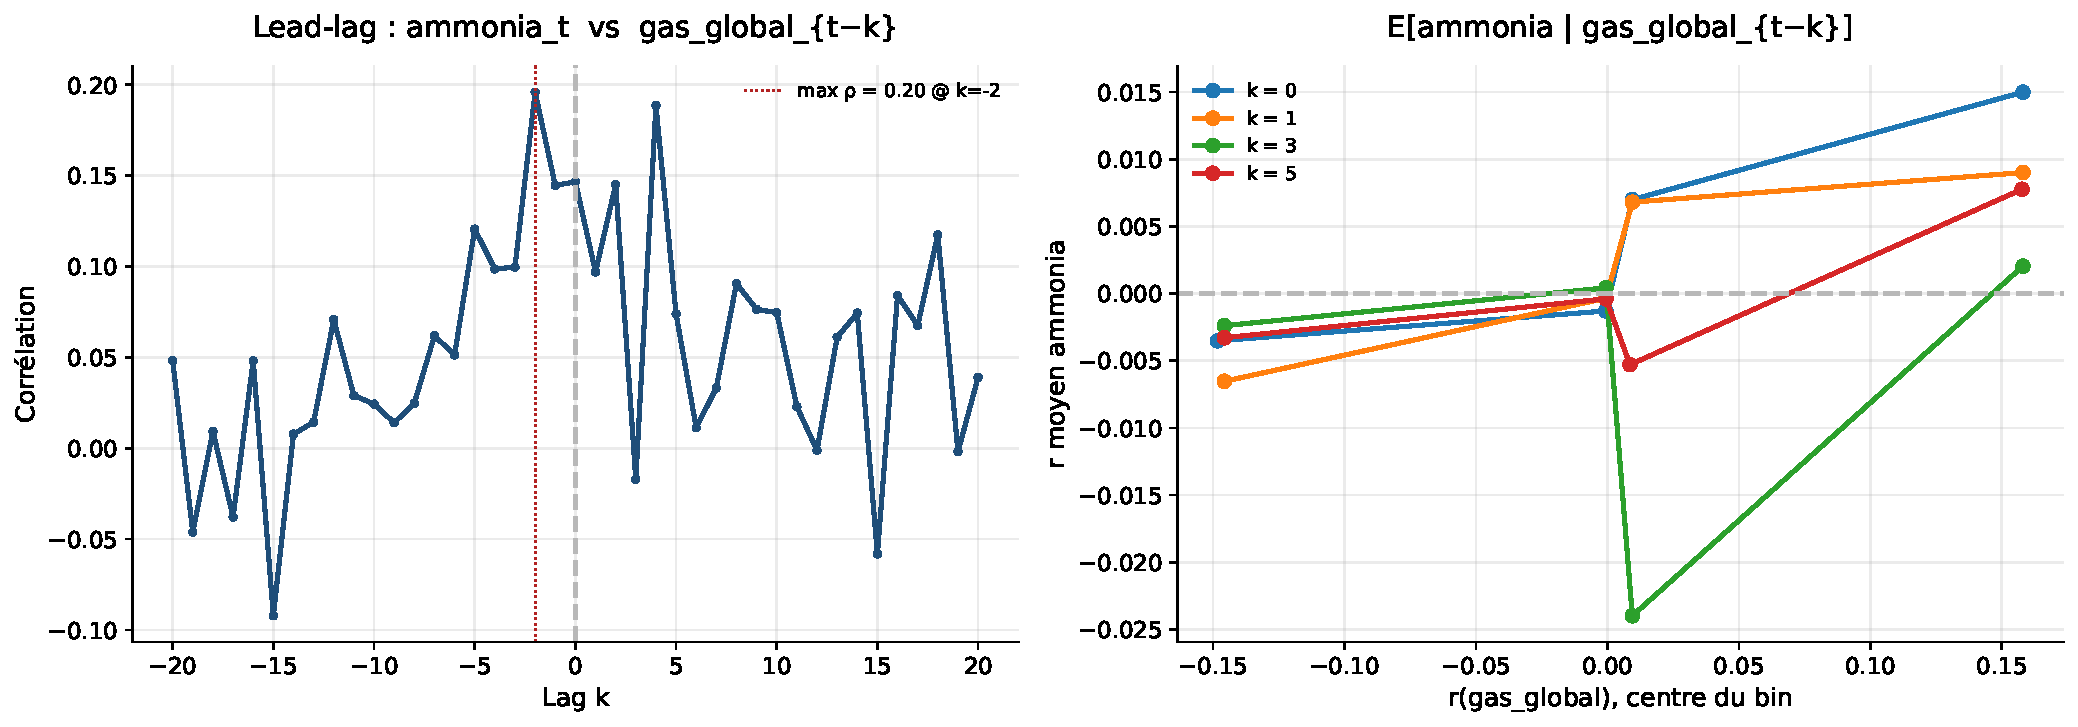
\includegraphics[width=0.48\linewidth]{leadlag_cond_gas_global.pdf}\hfill
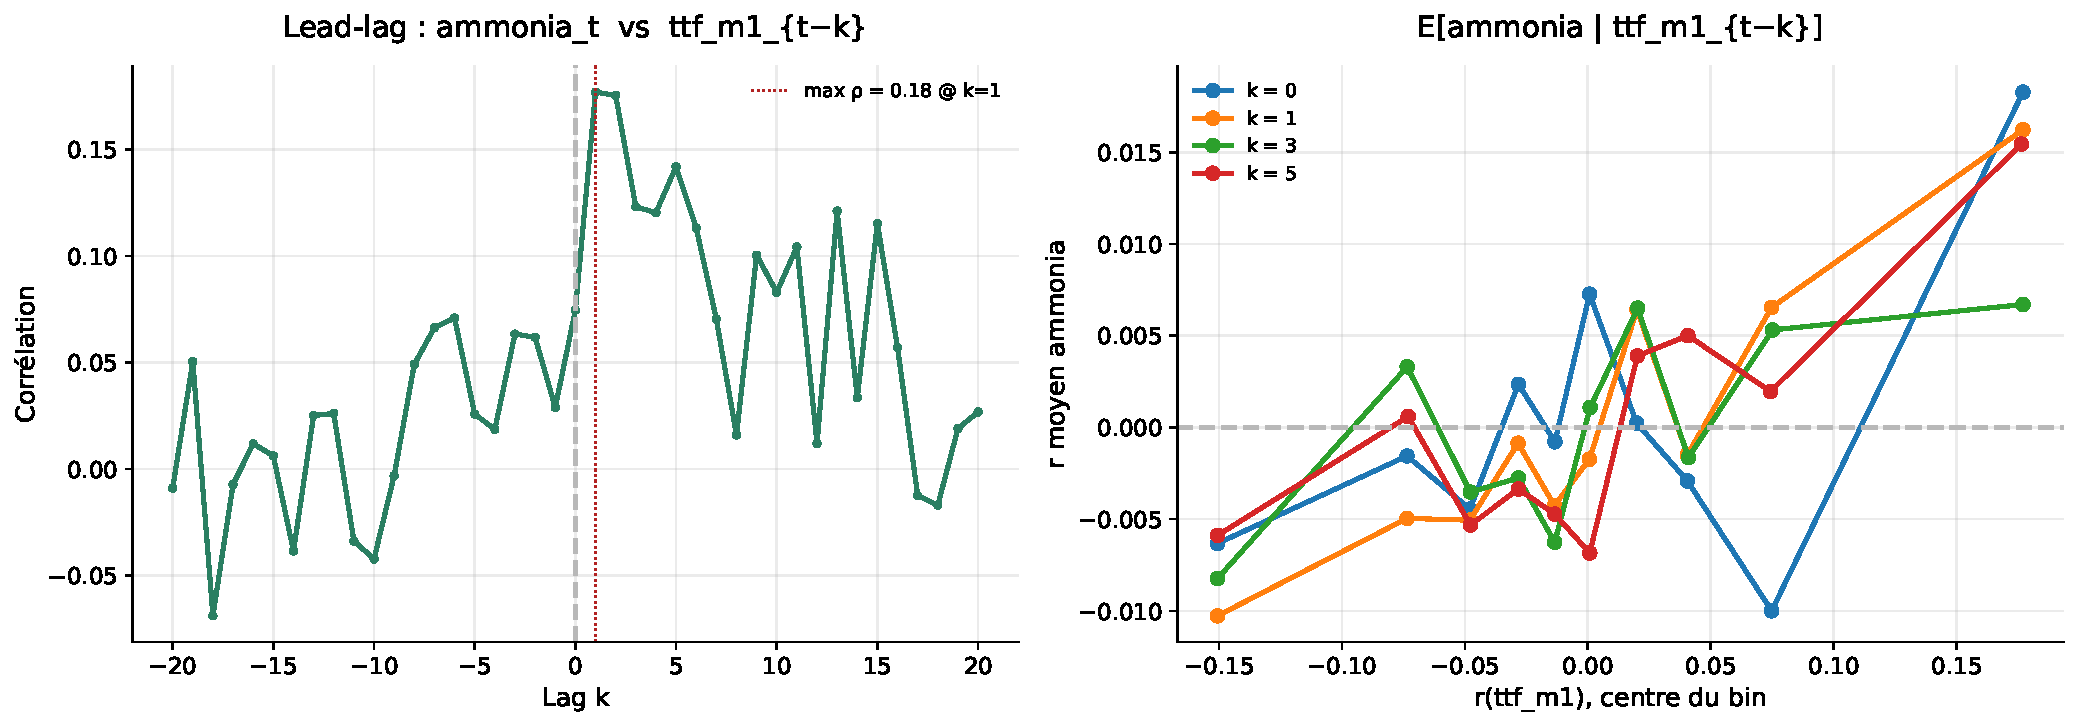
\includegraphics[width=0.48\linewidth]{leadlag_cond_ttf_m1.pdf}
\caption{Lead-lag and conditional expectation diagnostics for the two retained candidates.}
\end{figure}

\begin{figure}[htbp]
\centering
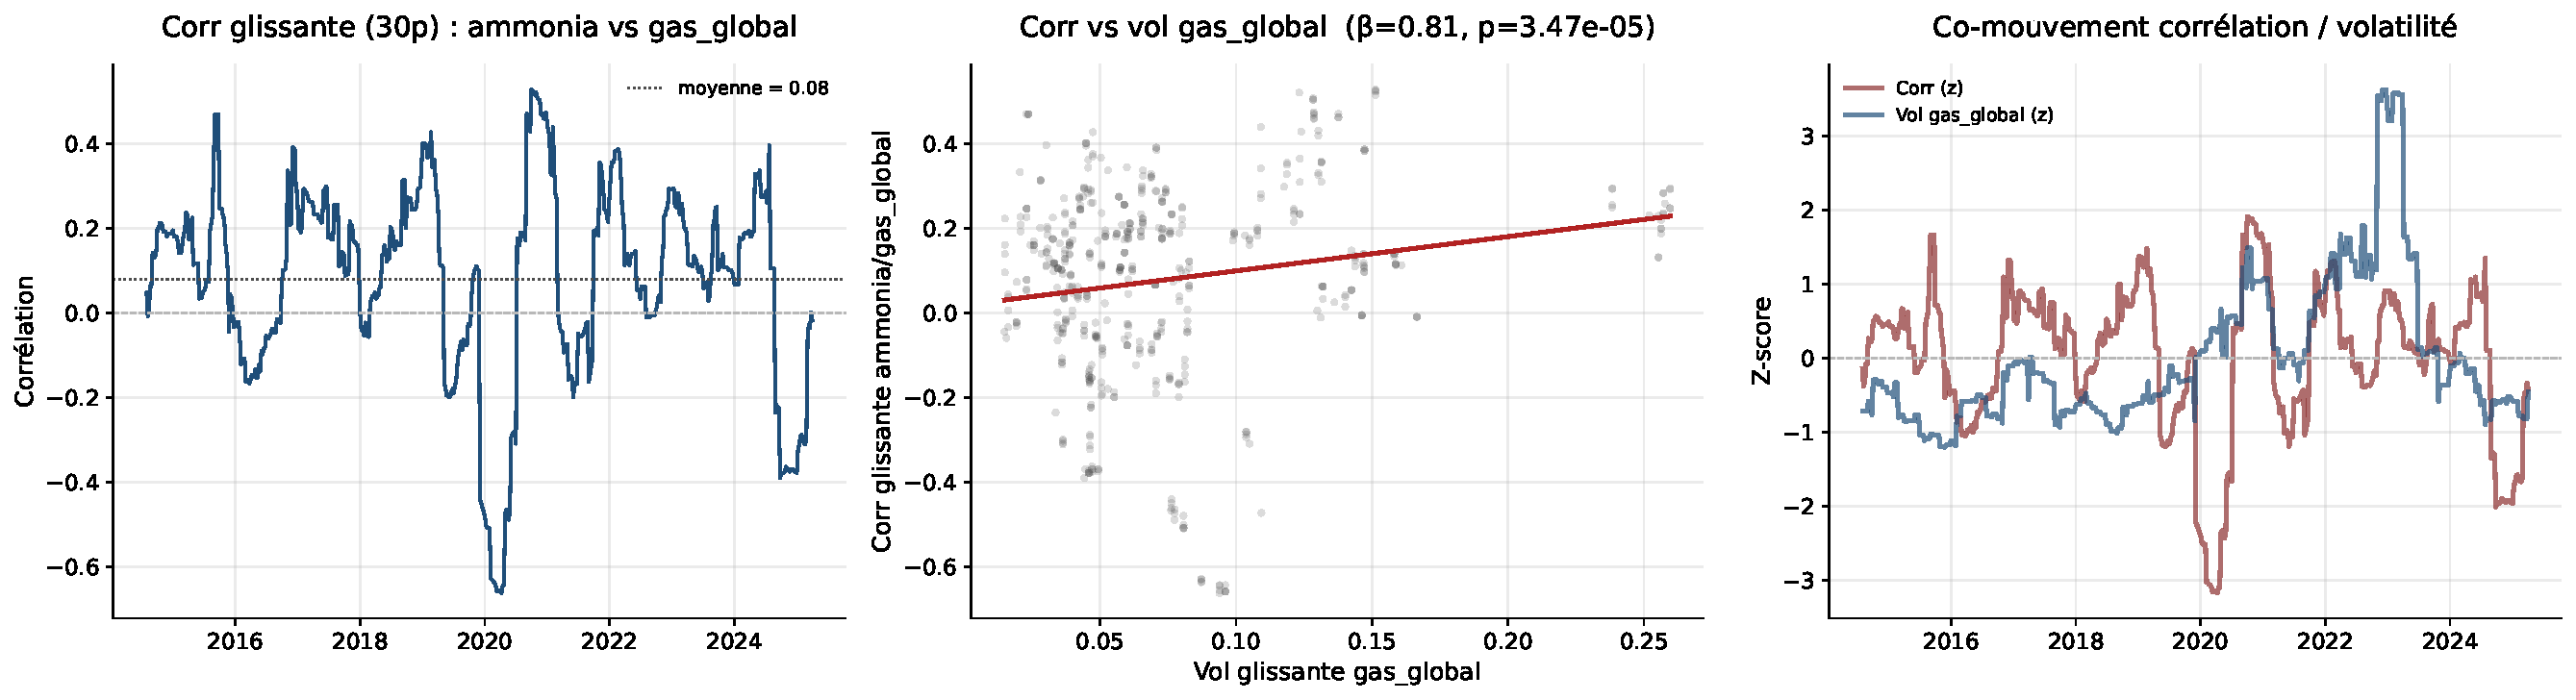
\includegraphics[width=0.48\linewidth]{rolling_corr_vol_gas_global.pdf}\hfill
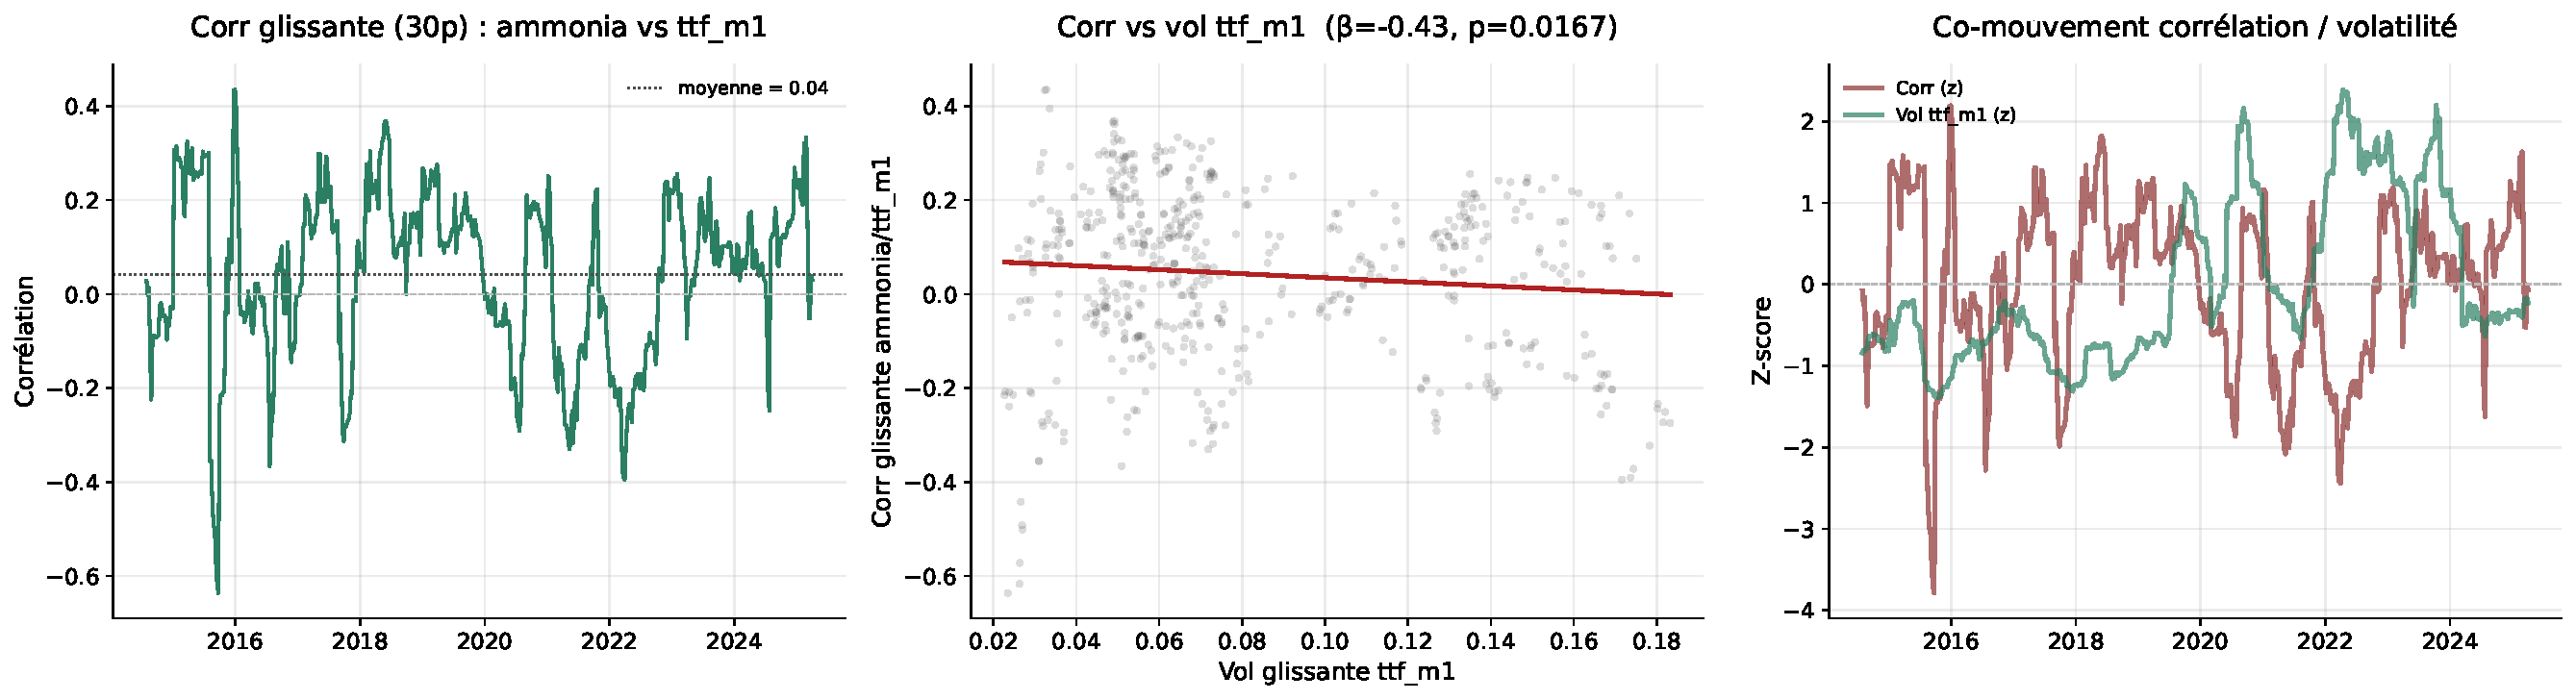
\includegraphics[width=0.48\linewidth]{rolling_corr_vol_ttf_m1.pdf}
\caption{Rolling correlation and correlation--volatility diagnostics for the two retained candidates.}
\end{figure}

\begin{figure}[htbp]
\centering
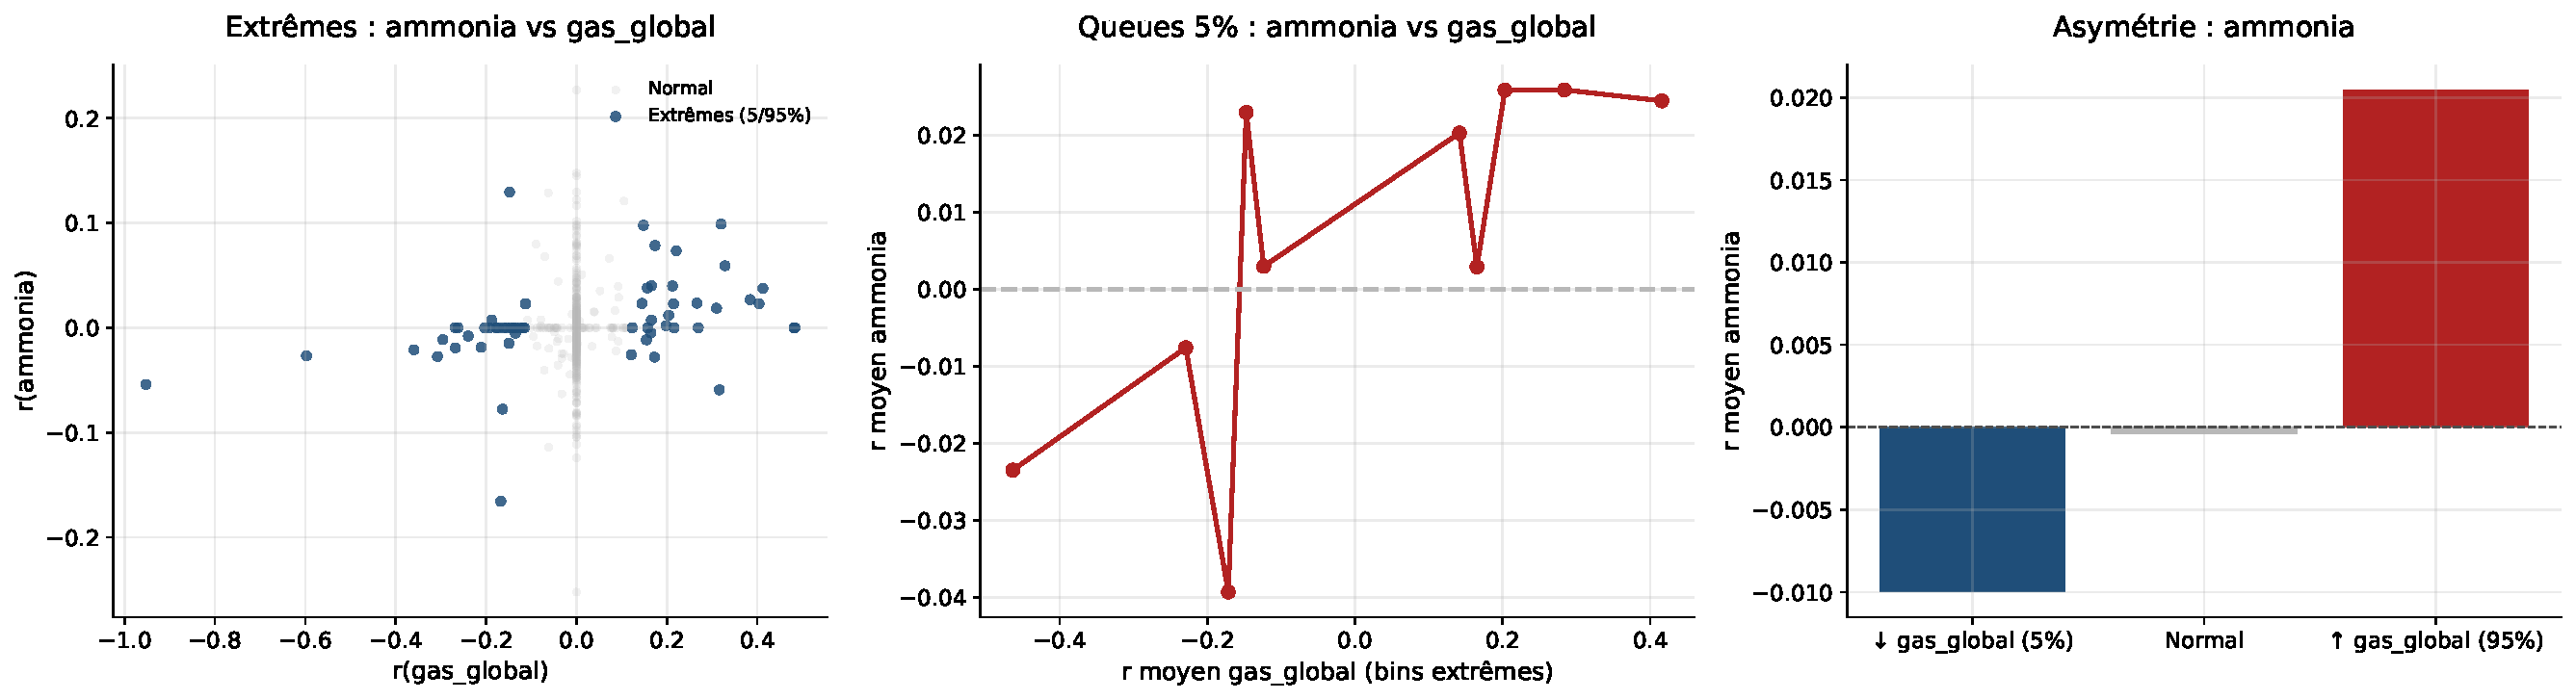
\includegraphics[width=0.48\linewidth]{extremes_gas_global.pdf}\hfill
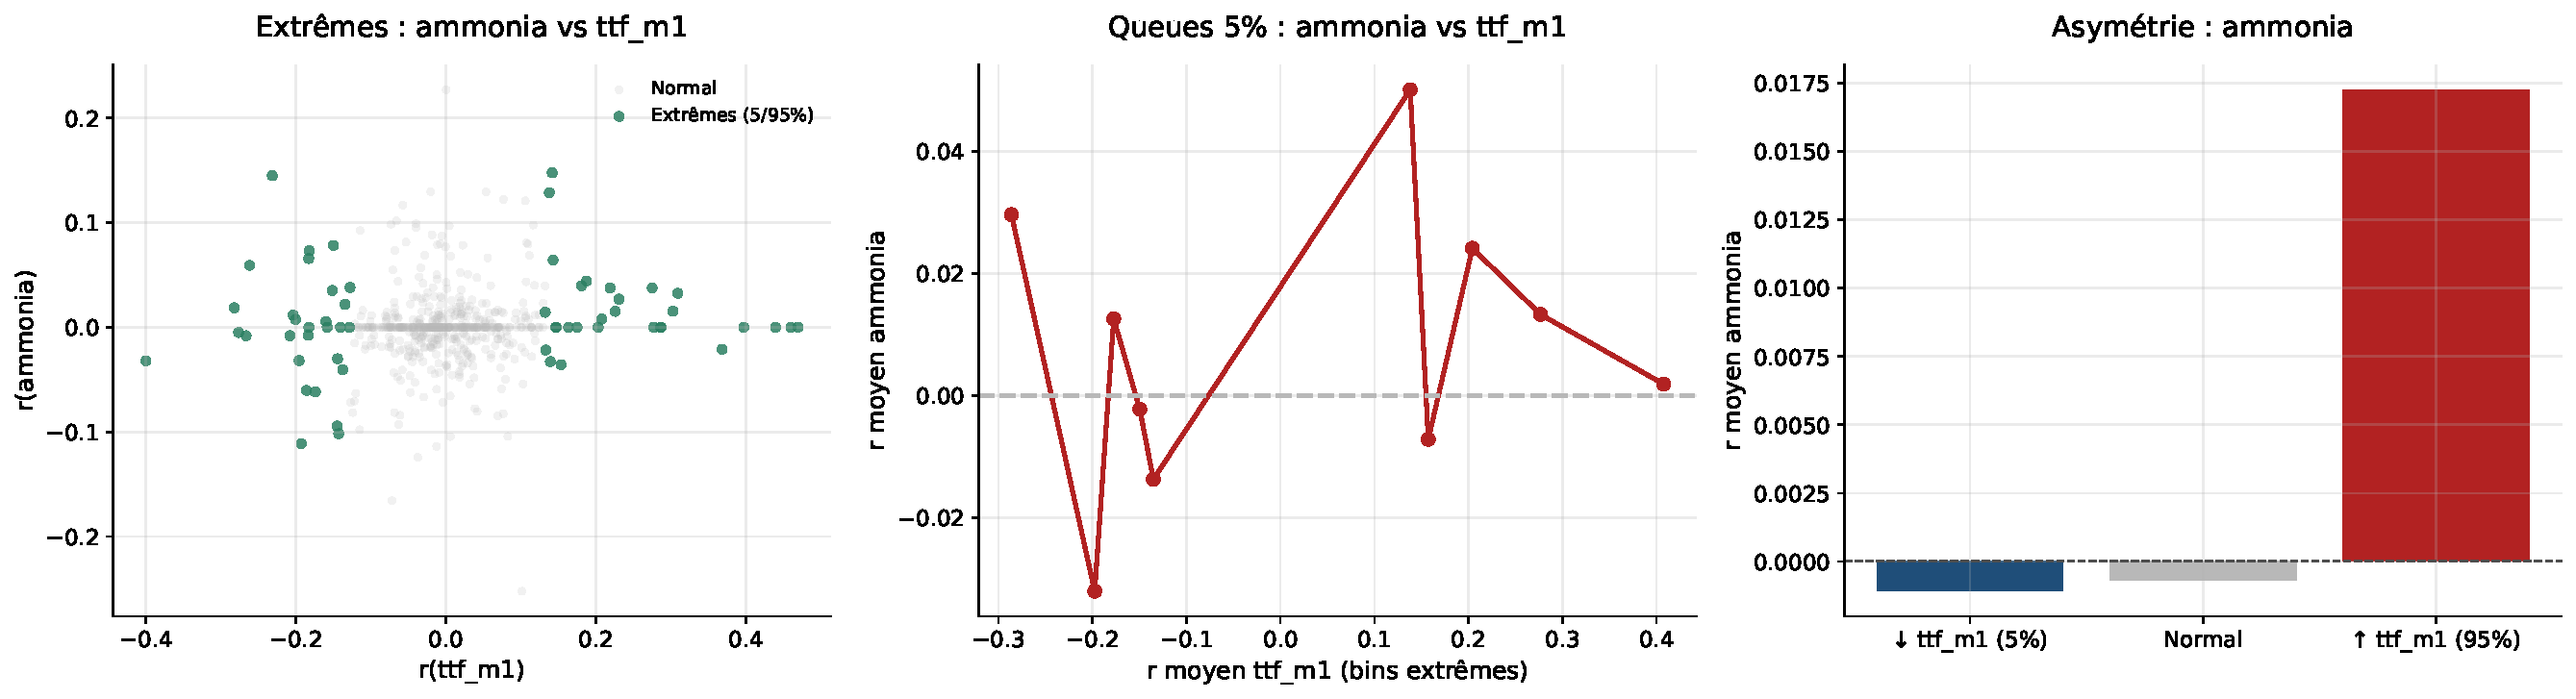
\includegraphics[width=0.48\linewidth]{extremes_ttf_m1.pdf}
\caption{Extreme-move diagnostics for the two retained candidates.}
\end{figure}
\subsection{Transmission trajectories}

\maybeplot{\figTransmission}{0.96}{
Multihorizon transmission trajectories. The curve \(\ell_j(k)=\Corr(r^A_t,r^j_{t-k})\) separates prospective interaction from contemporaneous or delayed co-movement.
}

The lead-lag curve separates explanatory co-movement from prospective interaction. A positive peak at \(k>0\) means that the proxy moves before ammonia. A peak at \(k<0\) means that ammonia moves before the proxy; that can be economically informative, but it is not directly hedgeable as a leading signal.

In the earlier fine analysis, \texttt{gas\_global} displayed a stronger contemporaneous or delayed relation: ammonia tended to move before the global gas proxy, with a peak around \(k=-2\). This supports a cost-regime reading rather than a clean leading-signal reading. By contrast, \texttt{ttf\_m1} showed a more credible short-horizon prospective signal, with a peak around \(k=1\). This is precisely the distinction the transmission trajectory is meant to identify.

\subsection{Focal horizons}

\maybeplot{\figFocal}{0.78}{
Focal transmission summary. Each instrument is summarized by the pair \((k_j^\star,L_j)\), where \(k_j^\star\) is the best prospective lag and \(L_j\) is the strength at that lag.
}

The focal plot compresses each trajectory into a timing coordinate and a strength coordinate. It is not a ranking by unconditional correlation. It is a ranking by prospective interaction.

This is important for proxy selection. A candidate with high contemporaneous correlation but weak prospective strength is less useful for cross-hedging than a candidate with smaller average correlation but a positive leading horizon. The empirical reading is therefore differentiated: \texttt{gas\_global} is useful for reading regimes, while \texttt{ttf\_m1} is the more natural short-horizon prospective candidate.

\subsection{Conditional response curves}

\maybeplot{\figResponse}{0.92}{
Conditional response curves. The curve \(m_j(u)=\E[r^A_t\mid r^j_{t-k_j^\star}\in B(u)]\) checks whether the relation has a shape beyond correlation.
}

The conditional response curve asks whether ammonia responds monotonically to the proxy. It is stricter than a correlation. A proxy can have a small correlation and still be useful if the response is concentrated in the right tail. Conversely, a proxy can have a nonzero correlation and still be unstable if the binned curve is erratic.

The gas proxies are most interesting in the upper part of the distribution. This is economically coherent. The industrial buyer is not symmetrically exposed to ammonia moves. The problematic event is an upward move in the cost of ammonia. A right-tail response is therefore more relevant than a symmetric average relation.

\subsection{Stress odds ratios}

\maybeplot{\figStressOdds}{0.78}{
Stress interaction measured by the tail odds ratio \(I_j\). Values above one indicate that proxy spikes and ammonia spikes co-occur more often than chance would suggest.
}

The stress odds ratio isolates a different object from the average correlation. It asks whether the proxy and ammonia become jointly extreme. If \(I_j>1\), the proxy has stress information. If \(I_j\simeq1\), proxy spikes are not especially informative for ammonia spikes.

The number of joint spikes matters. A high odds ratio with very few joint events should be read as suggestive, not conclusive. This is one reason why the stress diagnostic is used as a selection aid, not as a standalone proof.

\subsection{Transmission regimes}

\maybeplot{\figRegimesGas}{0.94}{
Two-axis interaction regimes for \texttt{gas\_global}. The left panel separates proxy stress from rolling transmission strength. The right panel reports the average future ammonia return in each quadrant.
}

The regime plot makes one distinction explicit:
\[
\text{proxy stress}
\neq
\text{transmitted proxy stress}.
\]
A gas market can be volatile without ammonia following it. Conversely, a moderate gas move can be informative if the current transmission strength is high.

For \texttt{gas\_global}, the fine analysis indicated that the ammonia-gas relation strengthens when gas volatility rises. That supports the interpretation of \texttt{gas\_global} as a regime proxy. For \texttt{ttf\_m1}, the earlier rolling correlation--volatility analysis suggested the opposite: the short-term predictive relation is more fragile when volatility rises. That supports the interpretation of \texttt{ttf\_m1} as a short-horizon signal whose reliability is state-dependent.

\subsection{Empirical synthesis}

The empirical analysis does not say that gas fully explains ammonia. It says something more precise.

\begin{center}
\renewcommand{\arraystretch}{1.15}
\begin{tabularx}{0.95\textwidth}{p{2.8cm}p{3.3cm}X}
\toprule
Instrument & Empirical role & Reading \\
\midrule
\texttt{gas\_global} & regime proxy & captures broad gas-cost conditions; more informative when the cost regime moves \\
\texttt{ttf\_m1} & short-horizon signal & carries the cleaner prospective timing; more fragile in stress \\
\texttt{ttf\_q1} & second-rank gas proxy & same economic channel, weaker short-term shape \\
Agriculturals & downstream proxies & economically linked but statistically weak for direct ammonia interaction \\
Equities & composite proxies & too many non-ammonia drivers for a clean cross-hedge signal \\
\bottomrule
\end{tabularx}
\end{center}

The conclusion of the interaction analysis is therefore:
\[
\texttt{gas\_global}
\quad\text{and}\quad
\texttt{ttf\_m1}
\]
are retained, but for different reasons. One reads regimes. The other carries timing.

\section{From interaction diagnostics to cross-hedging}

\subsection{Candidate selection}

A cross-hedge should not be estimated before the interaction structure has been identified. The diagnostics above decide which instruments can enter the hedge vector and how their role should be interpreted.

Let
\[
Y_t=r^A_{t+1}
\]
be the future ammonia return to be hedged, and let
\[
Z_t
=
\left(
r^{j_1}_t,\ldots,r^{j_m}_t
\right)^\top
\]
be the vector of retained proxy returns. In this application, the natural first choice is
\[
Z_t
=
\left(
r^{\mathrm{gas\_global}}_t,
r^{\mathrm{ttf\_m1}}_t
\right)^\top .
\]

The point is not that these two instruments are perfect. The point is that they survive different interaction tests. \texttt{gas\_global} is retained because it captures broad cost-regime information. \texttt{ttf\_m1} is retained because it has a more credible short-horizon prospective link.

\subsection{Dynamic hedge design}

A dynamic hedge is a predictable vector $h_t \in \mathbb{R}^m$, chosen using the information available at date $t$. The hedged one-period ammonia return is
\[
Y_t - h_t^\top Z_t.
\]
The standard minimum-variance hedge chooses $h_t$ to minimize the conditional variance of this residual exposure:
\[
h_t^\star
=
\arg\min_{h \in \mathbb{R}^m}
\mathbb{E}
\left[
\left(Y_t-h^\top Z_t\right)^2
\mid
\mathcal F_t
\right],
\]
where $\mathcal F_t$ denotes the information available at date $t$, including past ammonia returns, past proxy returns, and the interaction diagnostics computed up to date $t$.

The interpretation is simple: $h_t^\star$ is the vector of hedge ratios that makes the residual ammonia exposure as small as possible in conditional mean-square error. If the $i$-th component of $h_t^\star$ is positive, the corresponding proxy is used to offset positive ammonia moves; if it is close to zero, the proxy contributes little to the hedge at that date.

In the rolling covariance implementation, define
\[
\widehat{\Sigma}_{ZZ,t}
=
\widehat{\mathrm{Var}}_t(Z_t),
\qquad
\widehat{\Sigma}_{ZY,t}
=
\widehat{\mathrm{Cov}}_t(Z_t,Y_t),
\]
where the estimates are computed on a rolling window ending at date $t$. The first-order condition of the quadratic minimization problem gives
\[
\widehat{\Sigma}_{ZZ,t} h_t
=
\widehat{\Sigma}_{ZY,t},
\]
and therefore
\[
h_t
=
\widehat{\Sigma}_{ZZ,t}^{-1}
\widehat{\Sigma}_{ZY,t},
\]
when $\widehat{\Sigma}_{ZZ,t}$ is invertible. This is the multivariate analogue of the usual hedge beta,
\[
\beta_t
=
\frac{\widehat{\mathrm{Cov}}_t(Y_t,Z_t)}
{\widehat{\mathrm{Var}}_t(Z_t)}.
\]

However, this covariance hedge should not be used mechanically. It only measures local linear co-movement. The interaction analysis shows that the retained proxies have different economic roles: $\mathrm{gas\_global}$ is mainly a cost-regime proxy, while $\mathrm{ttf\_m1}$ is mainly a short-horizon prospective signal. Therefore, the hedge should not only estimate a direction; it should also decide when that direction is reliable.

A simple interaction-aware hedge can be written as
\[
h_t^{\mathrm{final}}
=
\omega_t g_t \widetilde h_t.
\]
Here, $\widetilde h_t$ is a smoothed version of the rolling covariance hedge, $g_t$ is an activation term measuring current transmission strength, and $\omega_t$ is a regime or stress intensity.

For example, one may define
\[
\widetilde h_t
=
(1-\lambda)\widetilde h_{t-1}
+
\lambda h_t,
\qquad
0<\lambda<1,
\]
in order to reduce excessive turnover and avoid reacting too strongly to noisy covariance estimates. 
A small $\lambda$ gives a more stable hedge and reduces turnover, but reacts slowly to changes in the covariance structure. A large $\lambda$ reacts faster, but is more exposed to estimation noise.

The activation term may be based on rolling prospective transmission, where the threshold $\ell_0$ controls the activation of the hedge through the current transmission strength:
\[
g_t
=
\mathbf 1_{\{L_t > \ell_0\}},
\qquad
L_t
=
\left[
\mathrm{Corr}_{t-W:t}
\left(
r^A_{s+1}, r^X_s
\right)
\right]_+,
\]
or, more smoothly,
\[
g_t
=
\min\left\{1,\frac{L_t}{\ell_0}\right\}.
\]
Thus the hedge is active only when the proxy is currently transmitting information to ammonia. A high threshold makes the hedge more selective and avoids acting when the ammonia--proxy link is weak. A low threshold keeps the hedge active more often, but increases the risk of hedging on a weak or unstable relation.


The stress intensity can be built from the two-axis regime diagnostic. If $\sigma^X_t$ denotes rolling proxy volatility and $L_t$ denotes rolling transmission strength, one may use
\[
\omega_t
=
1
+
\gamma
\mathbf 1_{\{\sigma^X_t > q_{0.75}(\sigma^X)\}}
\mathbf 1_{\{L_t > q_{0.75}(L)\}},
\qquad
\gamma \ge 0.
\]
Where the stress parameter $\gamma$ controls the amplification of the hedge in high-stress/high-transmission regimes. A larger $\gamma$ gives more protection when proxy stress is transmitted to ammonia, but also increases exposure to proxy-specific noise.

This increases hedge intensity precisely in the high-stress/high-transmission regime, where proxy stress is most likely to be transmitted to ammonia.

The resulting rule keeps the covariance hedge as a baseline direction, but it prevents the hedge from being active merely because a proxy is economically plausible. The hedge is strengthened when the proxy is both statistically connected to ammonia and currently in a regime where this connection is transmitted.

\subsection{Limitations}

Three limitations are structural.

First, ammonia prices are physical benchmark prices. They contain logistics, contract structure, regional basis and marginal-source effects that are not fully observed in financial time series.

Second, tail diagnostics are sample-sensitive. A stress odds ratio is informative only if the number of joint tail observations is reported and interpreted cautiously.

Third, gas exposure is not the same as ammonia exposure. Gas explains part of the production-cost channel, but not the full delivered benchmark. Cross-hedging should therefore be read as partial risk reduction, not replication.

\section{Conclusion}

Ammonia is not a gas derivative. It is a physical commodity whose price is formed through feedstock costs, delivered logistics, benchmark geography, marginal supply and downstream demand. Gas is the natural first proxy because it enters hydrogen production directly, but that fact alone is not enough to justify a hedge.

The interaction diagnostics separate several ideas that are often collapsed into one correlation. Multihorizon transmission identifies timing. Focal horizons summarize prospective strength. Conditional response curves reveal shape. Tail odds ratios isolate stress co-occurrence. Two-axis regimes distinguish volatile proxies from transmitted proxy stress.

The empirical reading is clear. \texttt{gas\_global} is best interpreted as a cost-regime proxy. \texttt{ttf\_m1} is best interpreted as a short-horizon prospective signal. The agricultural and equity candidates are economically connected but empirically weaker or too composite for a clean ammonia proxy.

Cross-hedging ammonia is therefore not first a beta-estimation problem. It is first an interaction-identification problem.

\appendix

\section{Additional screening figures}

\begin{figure}[htbp]
\centering
\begin{subfigure}{0.48\linewidth}
\centering
\includegraphics[width=\linewidth]{\figScatterTTFQ}
\caption{\texttt{ttf\_q1}}
\end{subfigure}
\hfill
\begin{subfigure}{0.48\linewidth}
\centering
\includegraphics[width=\linewidth]{\figScatterYara}
\caption{\texttt{yara}}
\end{subfigure}
\caption{Second-rank and composite candidates.}
\end{figure}

\begin{figure}[htbp]
\centering
\begin{subfigure}{0.48\linewidth}
\centering
\includegraphics[width=\linewidth]{\figScatterOrica}
\caption{\texttt{orica}}
\end{subfigure}
\hfill
\begin{subfigure}{0.48\linewidth}
\centering
\includegraphics[width=\linewidth]{\figScatterCorn}
\caption{\texttt{corn}}
\end{subfigure}
\caption{Equity and agricultural candidates.}
\end{figure}

\begin{figure}[htbp]
\centering
\begin{subfigure}{0.48\linewidth}
\centering
\includegraphics[width=\linewidth]{\figScatterWheat}
\caption{\texttt{wheat}}
\end{subfigure}
\hfill
\begin{subfigure}{0.48\linewidth}
\centering
\includegraphics[width=\linewidth]{\figScatterSoybeans}
\caption{\texttt{soybeans}}
\end{subfigure}
\caption{Downstream agricultural candidates.}
\end{figure}

\begin{figure}[htbp]
\centering
\includegraphics[width=0.55\linewidth]{\figScatterRice}
\caption{Downstream agricultural candidate: \texttt{rice}.}
\end{figure}


\newpage

\begin{thebibliography}{9}

\bibitem{ifa}
International Fertilizer Association,
\emph{Public Summary Short-Term Fertilizer Outlook 2024--2025}.

\bibitem{yarahandbook}
Yara,
\emph{Fertilizer Industry Handbook 2025}.

\bibitem{cf}
CF Industries,
\emph{Annual Report 2023}.

\bibitem{yarair}
Yara,
\emph{Integrated Report 2024}.

\bibitem{nutrien}
Nutrien,
\emph{Fourth Quarter and Full-Year 2024 Results}.

\bibitem{fertiglobe}
Fertiglobe,
\emph{Q4 2024 Financial Results Press Release}.

\bibitem{platts}
S\&P Global Commodity Insights,
\emph{Specifications Guide: Global Fertilizers, January 2026}.

\bibitem{argus}
Argus Media,
\emph{Argus Ammonia Methodology}.

\bibitem{cbam}
European Commission,
\emph{Carbon Border Adjustment Mechanism}.

\bibitem{tanguy}
Hervé Tanguy,
\emph{Stratégie concurrentielle dans les industries de commodités},
\emph{La Jaune et la Rouge}, n\textsuperscript{o} 678, octobre 2012.

\end{thebibliography}

\end{document}
